% !TeX root = ../main.tex
\chapter{相机和图像}
\section{相机模型}
视觉SLAM本质上是对空间点,相机位姿的求解。SLAM系统的输入是时序的图片,因此我们有必要了解一下现实中的三维信息是如何被转化成图片上一个个像素点的。我们通过对相机的建模,来模仿现实相机的行为,从而帮助我们理解相机的工作原理。现在我们就来介绍一种最常用的相机模型:\textbf{针孔相机模型(Pinhole camera)}
\subsection{针孔相机模型}
针孔相机模型模型描述的是一束光线通过针孔之后,在针孔背后投影成像。由于获得好的成像效果,我们在相机的前方加了透镜。透镜的加入对成像过程中光线的传播会产生新的影响:一是透镜自身的形状对光线传播的影响,二是在机械组装过程中,透镜和成像平面不可能完全平行,这也会使得光线穿过透镜投影到成像平面时的位置发生变化。这个现象叫做畸变,因此在使用相机前,对测量精度较高的相机,还要做非线性标定,即测出畸变参数。因此我们的建模分成两部分:对针孔模型的建模和对相机畸变的建模。
\begin{figure}
	\centering
	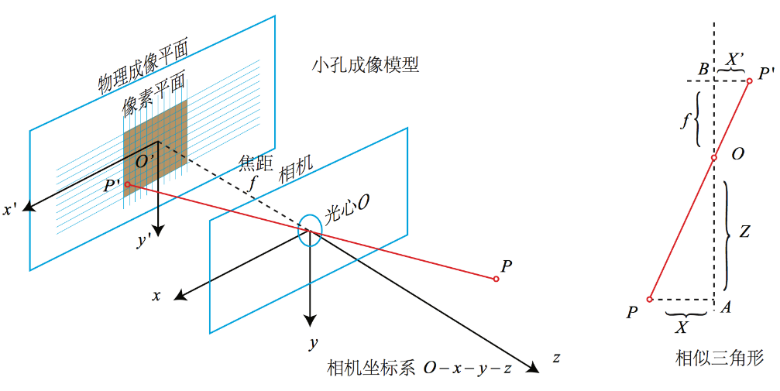
\includegraphics[height=5cm]{figures/pinholemodule.png}
	\caption{针孔模型}
\end{figure}
下面我们对这个针孔模型进行几何建模。设O–xyz为相机坐标系,现实世界中的空间点P,经过小孔O投影之后,落在成像平面O'-x'y'z'上,为P'。设P,P'的坐标分别为$[X,Y,Z]^{T},\left[X^{\prime}, Y^{\prime}, Z^{\prime}\right]^{T}$,成像焦距为f。那么根据三角形相似,则有:
\begin{equation*}
\frac{Z}{f}=-\frac{X}{X^{\prime}}=-\frac{Y}{Y^{\prime}}
\end{equation*}
这里的负号表示成的是倒立的像。为了简化计算,我们常常会把这个负号去掉,把成像平面对称至相机前方:
\begin{equation}
\frac{Z}{f}=\frac{X}{X^{\prime}}=\frac{Y}{Y^{\prime}}\label{Ptochengxiang}
\end{equation}
式\ref{Ptochengxiang}描述了空间点P经过小孔成的像之间的空间几何关系。但是在相机坐标系中,我们需要的是像素点的坐标,所以我们需要进一步变换。\par
设成像平面上的像素平面O–uv,则像素平面上点P'的像素坐标为:$[u, v]^{T}$。像素坐标系定义方式:原点位于图像成像平面左上角,$u$轴x轴平行且与向右,$v$轴与y平行且向下。在像素坐标系和成像平面之间通常相差了一个\textbf{缩放}和一个\textbf{原点的平移},我们设像素坐标在轴上缩放了$\alpha$倍,在轴上缩放了$\beta$倍,同时原点平移了$\left[c_{x}, c_{y}\right]$。这样我们就得到了像素坐标系和成像平面的关系,那么P'的成像坐标和其像素坐标关系如下:
\begin{equation}
\left\{\begin{array}{l}{u=\alpha X^{\prime}+c_{x}} \\ {v=\beta Y^{\prime}+c_{y}}\end{array}\right.
\label{chengxiangtopixel}
\end{equation}
将\ref{Ptochengxiang}代入上式子,并且将$\alpha f$合成为$f_x$,将$\beta f$合成为$f_y$得:
\begin{equation}
\left\{\begin{array}{l}{u=f_{x} \frac{X}{Z}+c_{x}} \\ {v=f_{y} \frac{Y}{Z}+c_{y}}\end{array}\right.
\end{equation}
写成矩阵的形式就是:
\begin{equation}
\left( \begin{array}{l}{u} \\ {v} \\ {1}\end{array}\right)=\frac{1}{Z} \left( \begin{array}{ccc}{f_{x}} & {0} & {c_{x}} \\ {0} & {f_{y}} & {c_{y}} \\ {0} & {0} & {1}\end{array}\right) \left( \begin{array}{l}{X} \\ {Y} \\ {Z}\end{array}\right) \triangleq \frac{1}{Z}\boldsymbol{KP}
\label{cameratopix}
\end{equation}
我们称上式中的\textbf{K}为相机的内参矩阵。一般来说,相机的内参在出厂之后是固定的,不会在使用过程中发生变化。有的厂商会告诉你相机的内参,而有时需要你自己确定相机的内参,也就是所谓的标定。可以看到,若三维空间内有一点$P=[x,y,z]$,先计算其在归一化平面上的坐标,也就是$[\frac{x}{z},\frac{y}{z},1]$,然后再乘以相机内参矩阵\textbf{K}就能得到像素位置。\par
现在我们来更深入的讨论一下这个流程。考虑一个世界坐标系下的点$P_w$,相机坐标系在世界坐标系下的位姿是$T$。公式\ref{cameratopix}中的$P$是相机坐标系下的坐标。因此若要计算$P_w$的像素坐标,需要先进行变换:
\begin{equation}
\left( \begin{array}{c}{u} \\ {v} \\ {1}\end{array}\right)=
\underbrace{
\left( \begin{array}{ccc}{f_{\alpha}} & {0} & {u_{0}} \\ {0} & {f_{\beta}} & {v_{0}} \\ {0} & {0} & {1}\end{array}\right)
\underbrace{\frac{1}{z_{c}}\overbrace{\left[ \begin{array}{cc}{\boldsymbol{R}} & {\boldsymbol{t}} \\ {\boldsymbol{0}^{T}} & {1}\end{array}\right]
\overbrace{\left( \begin{array}{c}{x_{w}} \\ {y_{w}} \\ {z_{w}} \\ {1}\end{array}\right)}^\text{世界坐标系}}^\text{相机坐标系}}_\text{归一化平面坐标}}_\text{像素平面坐标}\label{totalequation}
\end{equation}
上式从相机坐标系变成归一化坐标系的过程中省略了第四维,方便起见,以后齐次坐标和非齐次坐标的转换不再指出。事实上,将式\ref{totalequation}中$\frac{1}{z_c}$去掉也无妨,因为对于齐次坐标同乘以一个非零的数,结果并不变,无非是最后像素坐标再同除最后一维即可。因此,上式可简单写成:
\begin{equation}
	\boldsymbol{P_{uv}=KTP_w}
\end{equation}
至此,针孔相机的成像我们便介绍清楚了。
\section{畸变}
\subsection{畸变的类型}
前面我们说道,为了获得好的成像效果,我们在相机的前方安装透镜,这就会产生了畸变。
其中,由于透镜形状引起的畸变称为径向畸变。在针孔模型中,一条直线投影到像素平面还是一条直线,可是在实际拍摄的照片中,直线往往会变成曲线,越靠近图像的边缘,这种现象越明显。由于实际加工制作的透镜往往是中心对称的,这使得不规则的畸变通常中心对称。它们主要分为两大类:桶形畸变和枕形畸变,如图\ref{jingxiangjibian}所示:
\begin{figure}
	\centering
	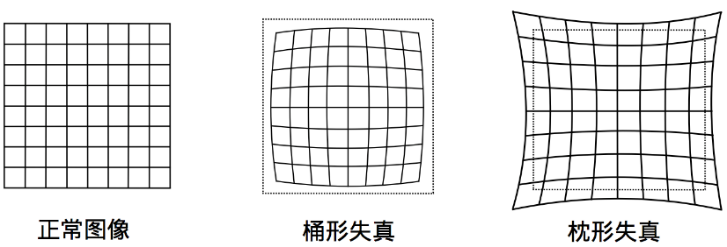
\includegraphics[height=4cm]{figures/jibian.png}
	\caption{径向畸变}\label{jingxiangjibian}
\end{figure}\par
除了透镜形状引起的畸变外,由于相机透镜安装的位置与成像平面不平行引起的畸变称之为切向畸变:
\begin{figure}
	\centering
	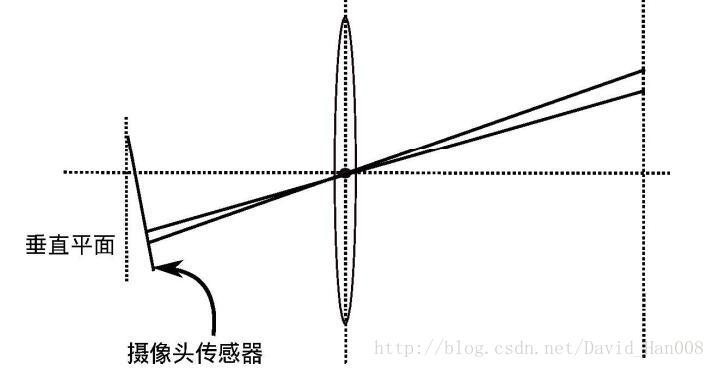
\includegraphics[height=4cm]{figures/qiexiangjibian.jpg}
	\caption{切向畸变}\label{qiexiangjibian}
\end{figure}\par
在SLAM特征点匹配过程中,这些错位的点是不可用的,我们要想办法去除掉畸变。我们知道平面上的任意一点p可以表示为$[x,y]^T$,也可以把它写成极坐标的形式$[r,\theta]^T$ ,其中$r$表示点$p$离坐标系原点的距离,$\theta$表示和水平轴的夹角。径向畸变可看成坐标点沿着长度方向发生了变化$\delta r$,也就是其距离原点的长度发生了变化。切向畸变可以看成坐标点沿着切线方向发生了变化,也就是水平夹角发生了变化$\delta \theta$。对于径向畸变,无论是桶形畸变还是枕形畸变,由于它们都是随着离中心的距离增加而增加。可以用一个多项式函数来描述畸变前后的坐标变化:这类畸变可以用和距中心距离有关的二次及高次多项式函数进行纠正:
\begin{equation}
\begin{aligned} x_{\text {corrected}} &=x\left(1+k_{1} r^{2}+k_{2} r^{4}+k_{3} r^{6}\right) \\ y_{\text {corrected}} &=y\left(1+k_{1} r^{2}+k_{2} r^{4}+k_{3} r^{6}\right) \end{aligned}
\end{equation}
其中$[x,y]^T$ 是未纠正的点的坐标,$[x_{corrected},y_{corrected}]^T$ 是纠正后的点的坐标,注意它们都是归一化平面上的点,而不是像素平面上的点。\par
对于畸变较小的图像中心区域,畸变纠正主要是k1起作用。而对于畸变较大的边缘区域主要是k2 起作用。普通摄像头用这两个系数就能很好的纠正径向畸变。对畸变很大的摄像头,比如鱼眼镜头,可以加入k3 畸变项对畸变进行纠正。\par
另一方面,对于切向畸变,可以使用另外的两个参数$p1 ,p2$来进行纠正:
\begin{equation}
\begin{aligned} c_{\text {corrected}} &=x+2 p_{1} x y+p_{2}\left(r^{2}+2 x^{2}\right) \\ y_{\text {corrected}} &=y+p_{1}\left(r^{2}+2 y^{2}\right)+2 p_{2} x y \end{aligned}
\end{equation}\par
对于相机坐标系中的一点$P(X,Y,Z)$,我们能够通过以下几个步骤找到这个点在像素平面上的正确位置:\par
\begin{enumerate}
\item 将三维空间点投影到归一化图像平面。设它的归一化坐标为$[x,y]^T$。
\item 对归一化平面上的点进行径向畸变和切向畸变纠正。
\begin{equation}
\begin{aligned} x_{\text {corrected}} &=x\left(1+k_{1} r^{2}+k_{2} r^{4}+k_{3} r^{6}\right)+2 p_{1} x y+p_{2}\left(r^{2}+2 x^{2}\right) \\ y_{\text {corrected}} &=y\left(1+k_{1} r^{2}+k_{2} r^{4}+k_{3} r^{6}\right)+p_{1}\left(r^{2}+2 y^{2}\right)+2 p_{2} x y \end{aligned}
\end{equation}
\item 将纠正后的点通过内参数矩阵投影到像素平面,得到该点在图像上的正确位置。
\begin{equation}
\begin{aligned} u &=f_{x} x_{\text {corrected}}+c_{x} \\ v &=f_{y} y_{\text {corrected}}+c_{y} \end{aligned}
\end{equation}
\item 在上面的纠正畸变的过程中,使用了五个畸变项。实际应用中,可以灵活选择纠正模型,对于畸变不大的情况,只选择k1 ,p1 , p2 这三项即可。
\end{enumerate}
我们从头来总结一下单目相机的成像过程:
\begin{enumerate}
\item 首先,世界坐标系下有一个固定的点$P$,世界坐标为$P_w$;
\item 相机坐标系的运动由$\vec{R},\vec{t}$或变换矩阵$\vec{T} \in SE(3)$描述。$P_w$的相机坐标为:$P_{c}=R P_{w}+t$;
\item 将$P_c$把它们投影到归一化平面$Z=1$上,得到$\tilde{P_c}=[X / Z, Y / Z, 1]^{T}$
\item 最后,$P_c$的归一化坐标经过内参变换后,得到它的像素坐标:$\vec{P_{uv}=K\tilde{P_c}}$ 。
\end{enumerate}\par
\subsection{相机的标定}
目前主流的相机标定方式是采用张友正标定法\cite{zhang1999flexible}。畸变参数一般在SLAM系统中是已知的,如果不知道的话,MATLAB和Opencv中都有封装好的相机标定的工具包,简单几步操作就能快速标定相机。